\chapter{Locality-Awareness}
\label{chapter:Locality-aware}

\begin{figure*}[tb]
	\centering
	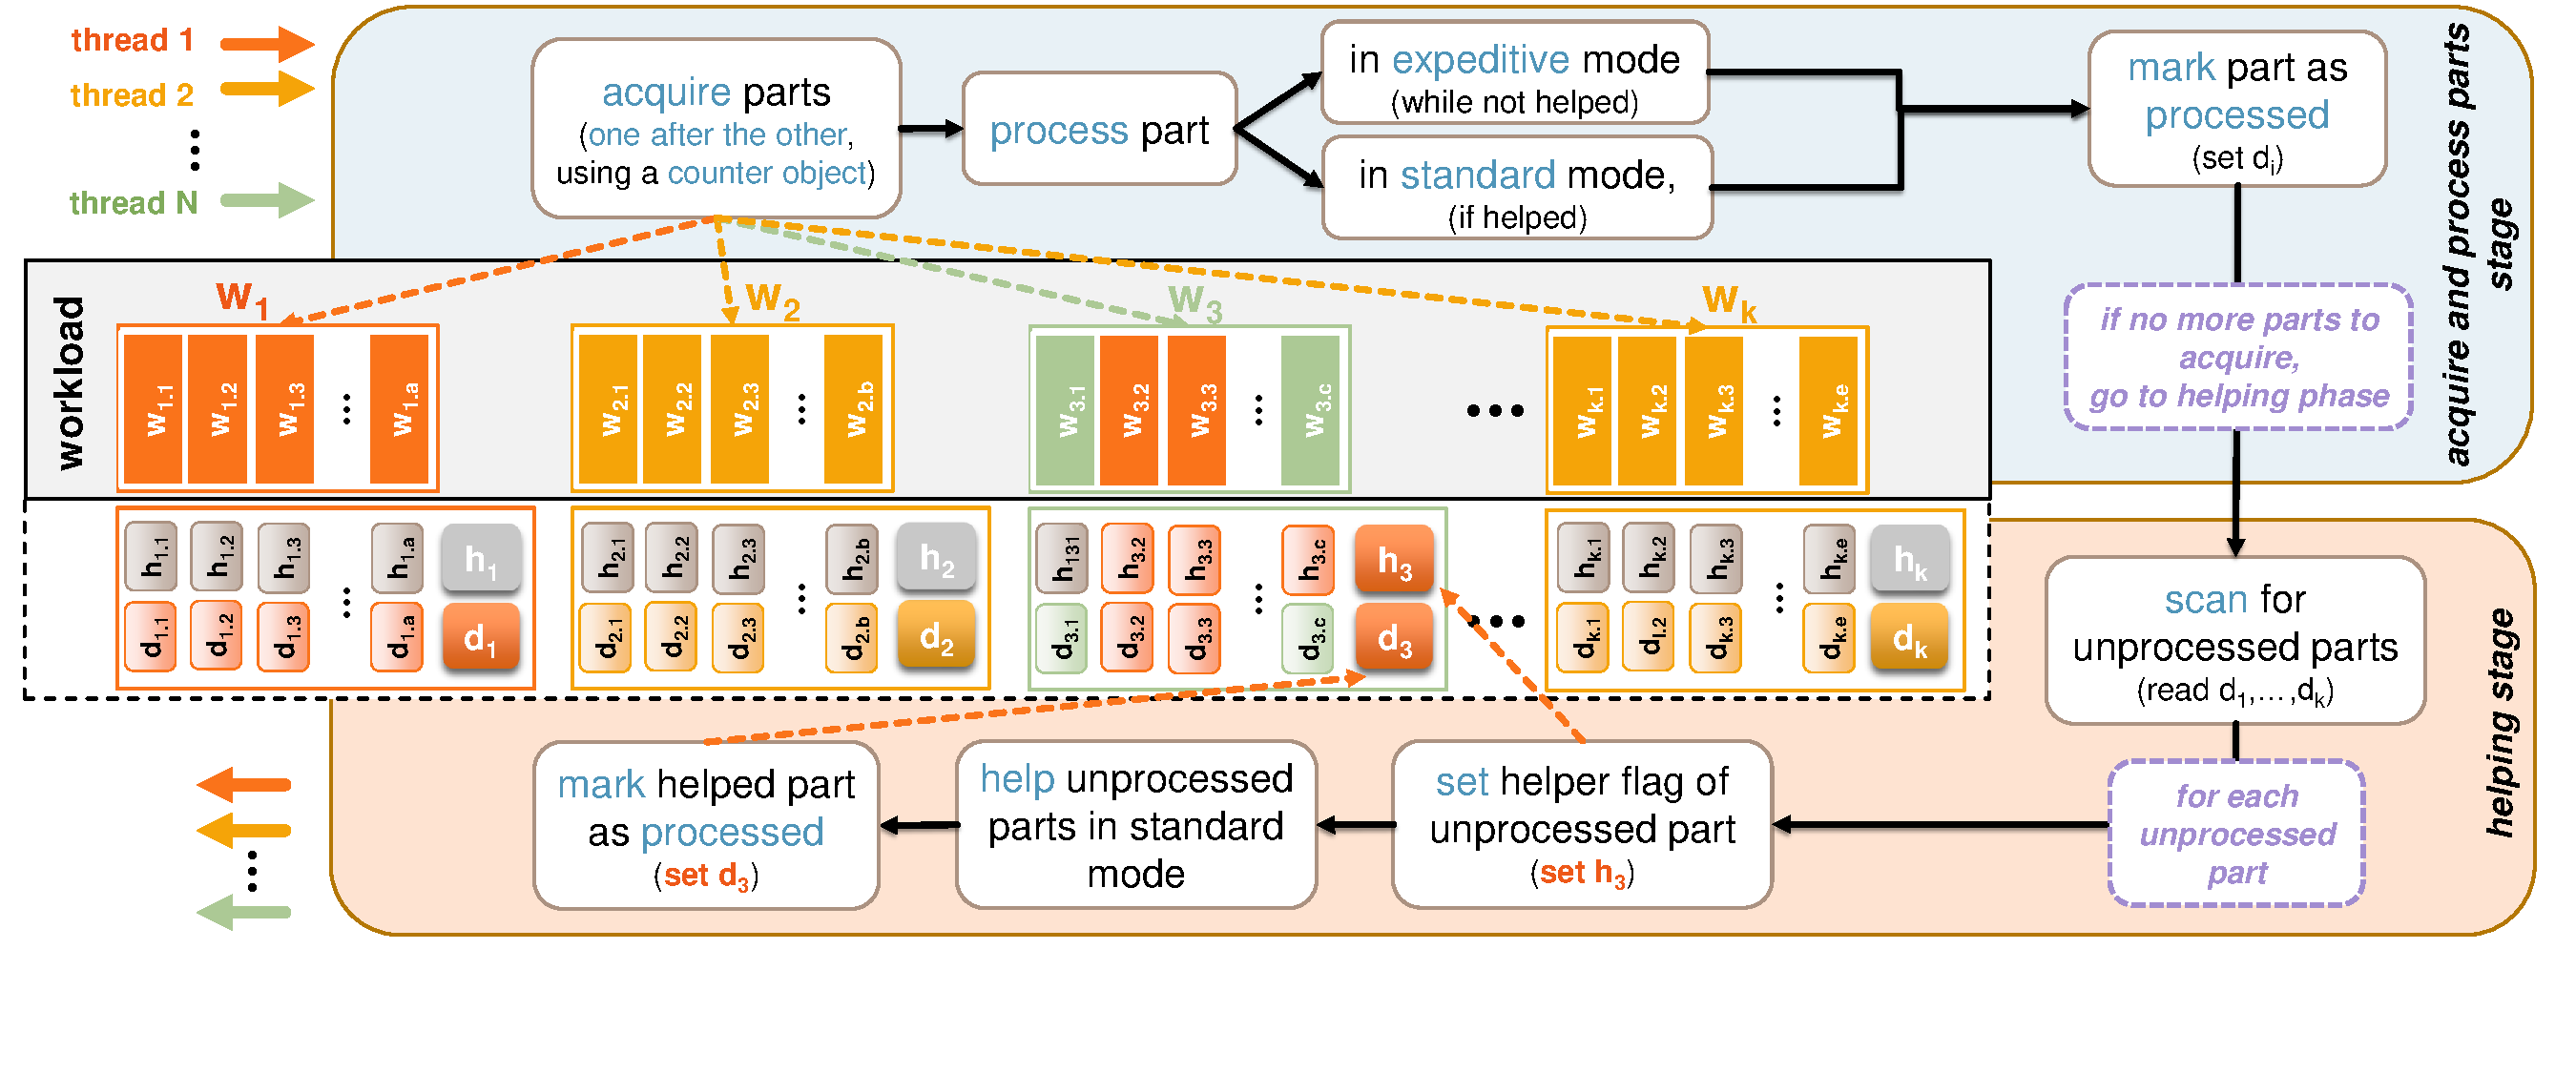
\includegraphics[width=0.9\textwidth]{figures/locality-aware/Refresh_ekosmas_2-Themis.pdf}	
	\vspace*{-0.8cm}
	\caption{Refresh flowchart.}
	\vspace*{-0.2cm}
	\label{fig:refresh:flowchart}
\end{figure*}


{\em Locality-awareness}  aims at capturing several design principles (Definition~\ref{def:principles})
for data series indexes which are crucial for achieving good performance.
A locality aware implementation respects these principles. 
% 
\begin{definition}
\label{def:principles}
Principles for {\em locality-aware} processing:
\begin{enumerate}
\item
{\bf Data Locality.} Separate the data into {\em disjoint sets} and have a distinct thread
processing the data of each set. This results in reduced communication 
cost (cache misses and branch misprediction) among the threads.
\item
{\bf High Parallelism \& Low Synchronization Cost.} 
Threads should work in parallel and independently from each other as much as possible. 
Whenever synchronization cannot be avoided, design the appropriate 
mechanisms to minimize its cost.
\item
{\bf Load Balancing.} Share the workload equally to the different threads, thus
avoiding load imbalances between threads and having all threads busy at each
point in time. 

\end{enumerate}
\end{definition}
% 
Enuring locality awareness results in good performance and is thus 
a desirable property for big data processing. In existing iSAX-based indexes, 
a thread operates on chunks of \textit{RawData} and processes disjoint sets of summarization
buffers and subtrees of the index tree. Also, an iSAX-based index employs 
several priority queues to store leaf nodes containing candidate series.
Thus, iSAX-based indexes are {\em locality-aware}.
% 
To describe \textit{ReFreSh} in more detail, consider a {\em blocking} locality-aware
implementation $\mathcal{A}$, which splits its workload into disjoint parts and assigns them to 
threads for processing. 
% 
The main idea behind it is to require from each thread that completes processing
its own workload,(instead of blocking, waiting for other threads to also finish), 
to scan for unprocessed workloads (e.g. in an iSAX-based index, unprocessed parts of $RawData$
or unprocessed summarization buffers), and help completing their processing. 

\textit{ReFreSh} (Algorithm~\ref{alg:refresh}) transforms $\mathcal{A}$ into a {\em lock-free} 
locality-aware implementation $\mathcal{B}$ that achieves high parallelism. 
% 
Let $W$ be the workload that $\mathcal{A}$ processes 
and let $w_1, \ldots, w_k$ be the parts it is separated to ensure locality awareness.
\textit{ReFreSh} applies for each data structure $D$ of $\mathcal{A}$, 
the following steps (depicted in Figure~\ref{fig:refresh:flowchart}):


%%%%%%%%%%%%%%%%%%%%%%%%%%%%%%% REFRESH ALGORITHM %%%%%%%%%%%%%%%%%%%%%%%%%%%%%%%%%%%%%% 

\begin{algorithm}[htbp]
    \footnotesize
    \vspace*{2mm}
    
    \begin{algorithmic}[1]
    
    \Procedure{InitializeSharedVariables}{}
        \State Workload part $\mathit{W} \gets [w_1, w_2, \ldots, w_k]$ \label{alg:refresh:w}
        \State Boolean array $\mathit{F} \gets [d_1, d_2, \ldots, d_k]$, initially $d_i = \False$ \label{alg:refresh:d}
        \State Boolean array $\mathit{H} \gets [h_1, h_2, \ldots, h_k]$, initially $h_i = \False$ \label{alg:refresh:h}
    \EndProcedure
    
    \vspace*{1mm}
    \State{Code for each thread:}    
    \vspace*{1mm}
    
    \Procedure{Refresh}{}
        \While{$\mathit{W}$ has available parts}  \label{alg:refresh:process:start}
            \State $\mathit{w_i} \gets$ Acquire an available part of $\mathit{W}$
            \State Mark $\mathit{w_i}$ as acquired
            \If{$h_i == \False$}  \label{alg:refresh:process:if}
                \State Process $\mathit{w_i}$ in expeditive mode, while checking that $h_i$ remains $\False$ \label{alg:refresh:process:expeditive}
                \State If $h_i == \True$, switch to standard mode
            \Else
                \State Process $\mathit{w_i}$ in standard mode \label{alg:refresh:process:standard}
            \EndIf
            \State $d_i \gets \True$ \label{alg:refresh:d:true}
        \EndWhile
        
        \vspace*{1mm}
        \ForAll{$d_i \in D$ where $d_i == \False$}  \label{alg:refresh:scan:ForAll} 
            \State Backoff()  \Comment{Avoid helping, if possible} \label{alg:refresh:help:backoff}
            \If{$d_i == \False$}  \label{alg:refresh:help:if}
                \State $h_i \gets \True$ \label{alg:refresh:h:true}
                \State Process $\mathit{w_i}$ in standard mode, checking periodically if $d_i$ remains $\False$ \label{alg:refresh:help:process}
                \State If $d_i == \True$, stop processing $\mathit{w_i}$
                \State $d_i \gets \True$ \label{alg:refresh:help:d:true}
            \EndIf
        \EndFor
    \EndProcedure
    
    \end{algorithmic}
    
    \caption{\textit{ReFreSh} - A general approach for transforming a blocking data structure $\mathit{D}$ into a lock-free one.}
    \label{alg:refresh}
\end{algorithm}

\newpage

\begin{enumerate}
    \item It attaches a {\em flag} $d_i$, $1 \leq i \leq k$, (initially \False)  
    with each $w_i$ to identify whether $w_i$'s processing is done.  
    As soon as a thread finishes processing $w_i$, it sets $d_i$ to \True\ (line~\ref{alg:refresh:d:true}).  

    \item Threads in $\mathcal{B}$ execute the same algorithm as in $\mathcal{A}$ to acquire parts of $W$ to process,  
    until all parts have been acquired (lines~\ref{alg:refresh:process:start}-\ref{alg:refresh:d:true}).  
    The thread that acquires a workload is its {\em owner}.  

    \item To achieve lock-freedom, every thread $t$, then, {\em scans} all the flags ($d_i$, $1 \leq i \leq k$)  
    to find those parts that are still unfinished (line~\ref{alg:refresh:scan:ForAll}).  

    \item Thread $t$ {\em helps} by processing, one after the other, each part found unfinished during scan.  
    For each part $w_i$, $1 \leq i \leq k$, that $t$ helps, it periodically checks $d_i$  
    to see whether other threads completed the processing of $w_i$. If this is so,  
    $t$ stops helping $w_i$ (line~\ref{alg:refresh:help:process}).  
    A thread that completes the processing of $w_i$ changes $d_i$ to \True\ (line~\ref{alg:refresh:help:d:true}).  

    \item Due to helping, every data structure $D$, employed in $\mathcal{A}$, may be  
    concurrently accessed by many threads. Thus, $\mathcal{B}$ should provide an efficient  
    lock-free implementation for all data structures of $\mathcal{A}$.  
\end{enumerate}


In locality-aware implementations, (e.g., in iSAX-based indexes), threads are expected to work
on their own parts of the data most of the time ({\em contention-free phase}), and they
may help other threads only for a small period of time at the end of their execution
({\em concurrent phase}).
In the contention-free phase, \textit{ReFreSh} avoids synchronization overheads incurred to
ensure lock-freedom. 
Specifically, it employs two implementations for each data strucutre $D$ of  $\mathcal{A}$,
one with low synchronization cost that does not support helping ({\em expeditive mode}),
and another that supports helping and has higher synchronization overhead ({\em standard mode}).  
To enable threads operate on the appropriate mode,  a {\em helping-indicator flag} $h_i$ 
(initially \False) , $1 \leq i \leq k$, is attached with each $w_i$. , which indicates whether 
$w_i$'s processing should be performed on expeditive or standard mode.
% 
A thread $t$ starts by processing its assigned workload 
on expeditive mode (lines~\ref{alg:refresh:h} and \ref{alg:refresh:process:if}-\ref{alg:refresh:process:expeditive}).
Before $t$ starts helping some part $w_i$, it sets $h_i$ to \True\ (line~\ref{alg:refresh:h:true}),
to alert $w_i$'s owner thread to start running on standard mode (line~\ref{alg:refresh:process:expeditive}).

To avoid helping whenever it is not absolutely necessary, i.e. when no thread has
failed (or is extremely slow), \textit{RefreSh} provides an optional {\em backoff scheme} that is used
by every thread $t$ (line~\ref{alg:refresh:help:backoff}) 
before it attempts to help other threads (line~\ref{alg:refresh:help:if}-\ref{alg:refresh:help:process}).
A small delay before switching to standard mode, often positively affects performance.
The delay is usually an estimate of the actual time a thread requires to finish its
current workload, calculated at run time.
% 
To minimize the work performed by a helper, \textit{ReFreSh} could
be applied  {\em recursively} by splitting each part $w_i$ to subparts. 
This way, a helper helps only the remaining unfinished subparts of $w_i$.
and not the whole $w_i$. Thus, the redundant work is further decreased. 
To achieve this, the subparts of $w_i$ should have their own flag and helping-indicator variables.

Lock-freedom is ensured due to the {\em helping code} (lines~\ref{alg:refresh:scan:ForAll}-
\ref{alg:refresh:help:d:true}), In \textit{ReFreSh}, only after a thread
$t$ processes a workload $w_i$, it sets $h_i$ to \True\, and $t$ performs 
the helping code after finishing with their assigned workloads. Thus, when $t$ completes
its helping code the processing of all parts of the workload has been completed. 
This means that $t$ may continue directly to the execution of the next stage, without
waiting for the other threads to complete the execution of the current stage. 
Therefore, this scheme renders the use of barriers useless, as needed to achieve lock-freedom. 

Summarizing, \textit{ReFreSh} is a general scheme for processing a locality-aware workload in a
lock-free way, without sacrificing locality-awareness. 

\bl{
\subsection{\textbf{ReFreSh with Dynamic Batches}}  

\textit{ReFreSh} is designed to be applied once per workload. Threads begin execution in 
\textit{expeditive mode} and switch to \textit{standard mode} when a helper arrives. However,
in an iSAX-based index, \textit{ReFreSh} is applied to multiple phases, including the
RawData array, summarization buffers, the iSAX tree, and the sorted arrays.  
When data arrives dynamically in batches, \textit{ReFreSh} must be applied separately for each phase
and its corresponding data structures. For data structures accessed only once per batch (e.g.,
the RawData array), this does not introduce issues. However, for data structures accessed
multiple times (e.g., summarization buffers and the iSAX tree), a challenge arises.  
% 
The core issue lies in how \textit{ReFreSh} determines when to switch execution modes.
Its behavior relies on boolean flags that initially have a value of \texttt{False} and transition
to \texttt{True} during processing. After processing the first batch, subsequent batches will
encounter these flags already set to \texttt{True}, causing \textit{ReFreSh} to always run
in \textit{standard mode}. This is suboptimal because \textit{standard mode} enables helping,
which is unnecessary unless a helper has actually arrived. To maintain performance,
\textit{ReFreSh} must be modified to support batch processing effectively.  

\subsubsection{\textbf{Modifications to Support Batches}}  

To ensure \textit{ReFreSh} works correctly with dynamic batches, we introduce the following
modifications:  

\begin{enumerate}  
    \item \textbf{Replacing Boolean Flags with Counters:}  
    Instead of using boolean flags, we replace them with counters. Each part $w_i$, where $1 \leq i
    \leq k$, is assigned a counter $d_i$ (initially set to 0). This counter tracks whether $w_i$ has
    completed processing for a specific batch. Once a thread finishes processing $w_i$, it
    sets $d_i$ to $\mathit{currentBatch} + 1$, which corresponds to the ID of the next
    batch (see Algorithm~\ref{alg:DRefresh}).  

    \item \textbf{Batch-Aware Execution of \textit{ReFreSh}:}  
    \textit{ReFreSh} is executed once per batch. Each time it runs, it requires the ID of the
    batch it is processing. The counter values are interpreted accordingly:  
    \begin{itemize}  
        \item A part $w_i$ is considered processed for a batch with ID $X$ when $d_i = X + 1$.  
        \item A helper has arrived at part $h_i$ for an update batch with ID $X$ when $h_i = X + 1$.  
    \end{itemize}  
\end{enumerate}  

By implementing these modifications, \textit{ReFreSh} maintains its efficiency across
multiple dynamic batches while ensuring that execution mode transitions occur only when necessary.


%%%%%%%%%%%%%%%%%%%%%%%%%%%%%%% Dynamic Refresh %%%%%%%%%%%%%%%%%%%%%%%%%%%%%%%%%%%%%%%%

\begin{algorithm}[htbp]
    \footnotesize
    \vspace*{2mm}
    
    \begin{algorithmic}[1]
    
    \State \textbf{Shared variables:}
    \State Workload part $\mathit{W} := \mathit{[w_1, w_2, \ldots, w_k]}$ \label{alg:DRefresh:w}
    \State \textbf{int} $\mathit{F} := \mathit{[d_1, d_2, \ldots, d_k]}$, initially $\mathit{d_i} = 0, \forall i \in [1, k]$ \label{alg:DRefresh:d}
    \State \textbf{int} $\mathit{H} := \mathit{[h_1, h_2, \ldots, h_k]}$, initially $\mathit{h_i} = 0, \forall i \in [1, k]$ \label{alg:DRefresh:h}
    
    \vspace*{1mm}
    \State \textbf{Code for each thread:}
    
    \Procedure{DRefresh}{int $\mathit{currentBatch}$}
        \While{$\mathit{W}$ has available parts} \label{alg:DRefresh:process:start}
            \State $\mathit{w_i} \gets$ acquire an available part of $\mathit{W}$
            \State Mark $\mathit{w_i}$ as acquired
            \If{$(\mathit{h_i} == \mathit{currentBatch})$ \textbf{or} $(\mathit{d_i} == \mathit{currentBatch}$ 
            \textbf{and} $\mathit{h_i} < \mathit{currentBatch})$} \label{alg:DRefresh:process:if}
                \State Process $\mathit{w_i}$ in expeditive mode, while checking the value of $h_i$ \label{alg:DRefresh:process:expeditive}
                \If{$\mathit{h_i} == \mathit{currentBatch} + 1$}
                    \State Switch to standard mode
                \EndIf
            \Else
                \State Process $\mathit{w_i}$ in standard mode   \label{alg:DRefresh:process:standard}
            \EndIf
            \If{$\mathit{d_i} == \mathit{currentBatch}$}
                \State $\mathit{CAS(\&d_i, currentBatch, currentBatch+1)}$ \label{alg:DRefresh:d:increase}
            \EndIf
        \EndWhile
        
        \ForAll{$\mathit{d_i} \in D$ where $\mathit{d_i} == \mathit{currentBatch}$} \label{alg:DRefresh:scan:ForAll} 
            \State Backoff to avoid helping if possible \label{alg:DRefresh:help:backoff}
            \If{$\mathit{d_i} == \mathit{currentBatch}$} \label{alg:DRefresh:help:if}
                \If{$\mathit{h_i} == \mathit{currentBatch}$} \label{alg:DRefresh:h:true}
                    \State $\mathit{CAS(\&h_i, currentBatch, currentBatch+1)}$ 
                \ElsIf{$\mathit{h_i} < \mathit{currentBatch}$}      \label{alg:DRefresh:h:fallenBehind}
                    \State \textbf{int} oldVal $\gets \mathit{h_i}$
                    \State $\mathit{CAS(\&h_i, oldVal, currentBatch+1)}$
                \EndIf
            \EndIf
            \State Process $\mathit{w_i}$ in standard mode, checking $\mathit{d_i}$
            \If{$\mathit{d_i} == \mathit{currentBatch}$}
                \State $\mathit{CAS(\&d_i, currentBatch, currentBatch+1)}$ \label{alg:DRefresh:help:d:true}
            \EndIf
        \EndFor
    \EndProcedure
    
    \end{algorithmic}
    
    \caption{Dynamic Refresh - A general approach for transforming a blocking data structure $\mathit{D}$ of a big-data application $\mathcal{A}$ into a lock-free one that supports dynamic insertions.}
    \label{alg:DRefresh}
    \end{algorithm}

    \newpage

    \begin{enumerate}
        \item As in \textit{ReFreSh}, threads acquire parts of the batch $W$ for processing until
        all parts have been claimed. Each thread must determine the appropriate processing mode.
        A helper has arrived at part $w_i$ if the value of $h_i$ is equal to the current batch ID + 1.
        The same applies to the processing of $d_i$. Once a thread finishes processing a part, it must
        atomically increment $d_i$ using a compare-and-swap (CAS) operation to ensure correctness, as
        multiple helpers may attempt to update it simultaneously (lines~\ref{alg:DRefresh:process:start}-
        \ref{alg:DRefresh:d:increase}).  
    
        \item To maintain lock-freedom, every thread $t$ scans all counters  
        ($d_i$, $1 \leq i \leq k$) to identify unfinished parts (line~\ref{alg:DRefresh:scan:ForAll}).  
    
        \item Thread $t$ {\em helps} by processing, one after another, each part that remains unfinished  
        after the scan. A part $w_i$ is considered unfinished when its corresponding $d_i$ value  
        is equal to the current batch ID. While processing, thread $t$ periodically checks $d_i$  
        to determine whether other threads have already completed $w_i$. For each part $w_i$ that $t$
        helps, it must announce that a helper has arrived by updating the value of $h_i$.  
        In the base case, where helping occurred for this part in the previous batch, $h_i$ is updated
        atomically using CAS (line~\ref{alg:DRefresh:h:true}). However, there are cases where $h_i$
        may lag behind for certain parts, as helping is not always required in every batch. For example,
        if a thread completes processing a part before a helper arrives, the corresponding $h_i$ value
        remains unchanged (line~\ref{alg:DRefresh:h:fallenBehind}). Once a thread finishes processing
        $w_i$, it attempts to update $d_i$ to the current batch ID + 1 
        (line~\ref{alg:DRefresh:help:d:true}).  
    \end{enumerate}
    
}